\documentclass{standalone}
\usepackage{mintikz}

\begin{document}
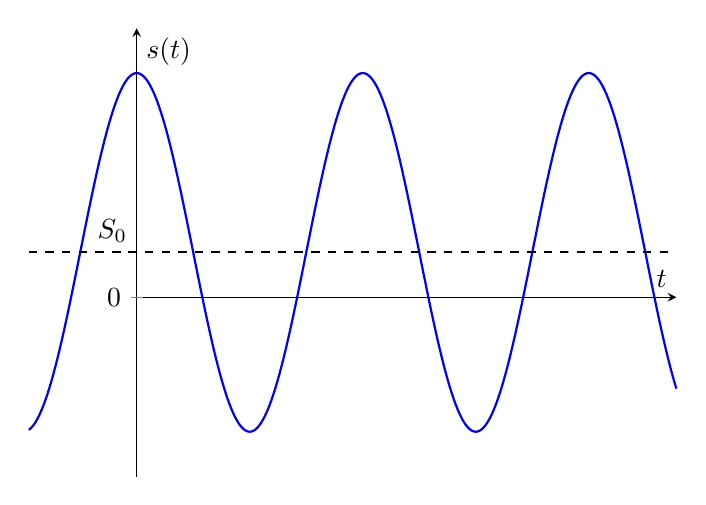
\begin{tikzpicture}[]
    \begin{axis}[
        xmin=0, xmax=15,
        ymin=-2, ymax=3,
        xtick={\empty},
        ytick={\empty},
        extra y ticks={0},
        xlabel=$t$, ylabel=$s(t)$,
        axis lines=center,
        clip=false]
        \addplot[
        domain=-3:15, samples=500,
        smooth, blue, thick]
        {.5+2*cos(deg(\x))};
        \addplot[
        domain=-3:15, thick,
        smooth, black, dashed]
        {.5};
        \node[anchor=south east] at (axis cs:0,.5) {$S_0$};
    \end{axis}
\end{tikzpicture}
\end{document}
